\section{การออกแบบส่วนการวิเคราะห์ ตรวจสอบ และแนะนำท่าทางของผู้ใช้}
ในการออกแบบส่วนการวิเคราะห์ ตรวจสอบ และแนะนำท่าทางของผู้ใช้ จะแสดงเป็นแผนภาพการทำงานระหว่างระบบต่าง ๆ ได้ ดังนี้
\begin{figure}
    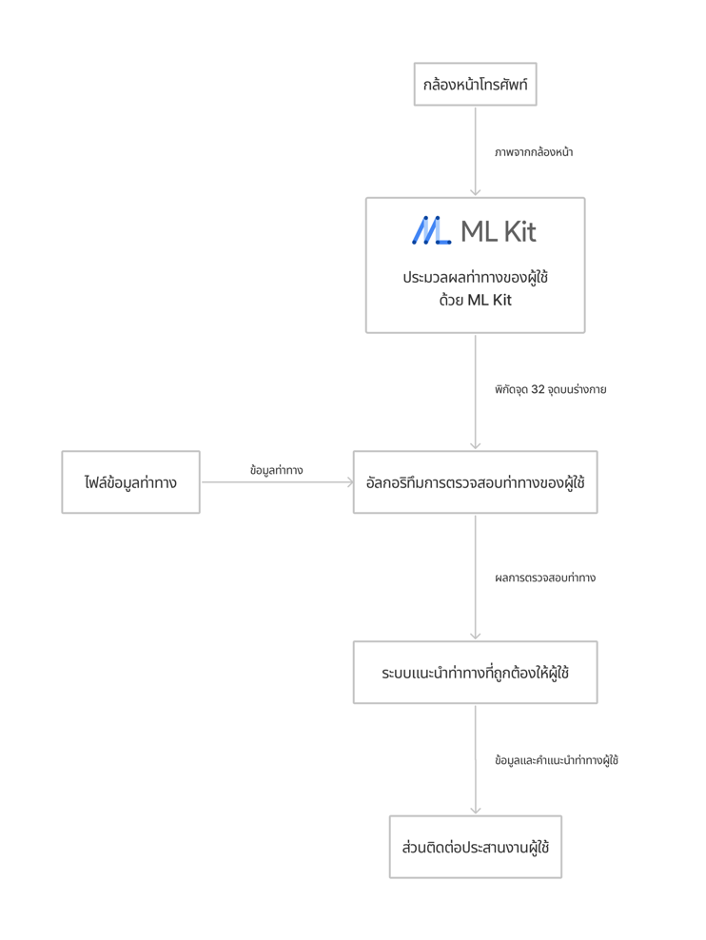
\includegraphics[width=\textwidth - 2cm]{chapter_3/pose overview.png}
    \caption{ภาพรวมระบบการวิเคราะห์ ตรวจสอบ และแนะนำท่าทางของผู้ใช้}
\end{figure}
จากแผนภาพข้างต้น สามารถอธิบายออกเป็นส่วนต่าง ๆ ซึ่งจะแบ่งออกเป็น 4 ส่วน คือ ส่วนการประมวลผลท่าทางของผู้ใช้ด้วย ML Kit, ส่วนไฟล์ข้อมูลท่าทาง, ส่วนอัลกอริทึมการตรวจสอบท่าทางของผู้ใช้ และส่วนระบบแนะนำท่าทางที่ถูกต้องให้ผู้ใช้

\subsection{ส่วนการประมวลผลท่าทางของผู้ใช้ด้วย ML Kit}
สำหรับระบบการวิเคราะห์ท่าทาง จะใช้ API ของ ML Kit ในการตรวจจับท่าทางของผู้ใช้ ซึ่งจะได้พิกัดจุดทั้งหมด 32 จุดทั่วร่างกาย
\begin{figure}
    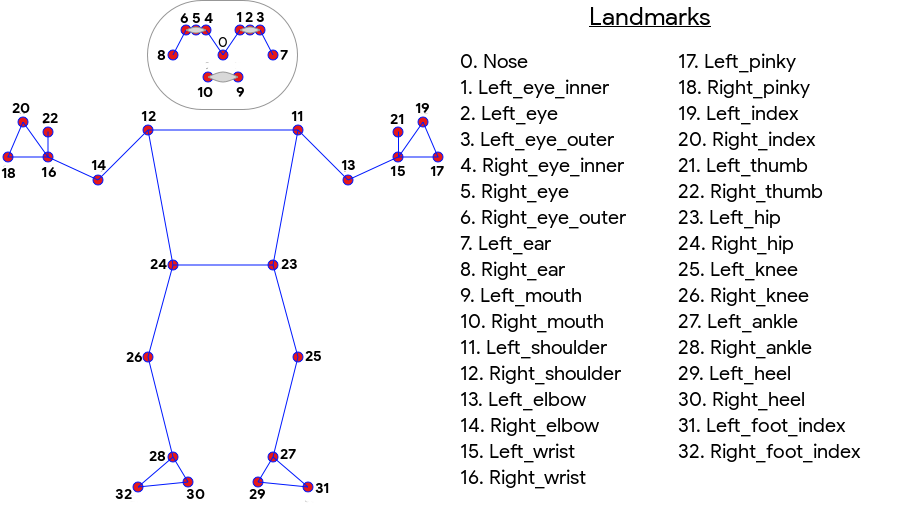
\includegraphics[width=\textwidth]{chapter_3/landmarks-fixed.png}
    \caption{แสดง Landmark จุดบนร่างกายที่ ML Kit สามารถตรวจจับได้}
\end{figure}

\subsection{ส่วนอัลกอริทึมการตรวจสอบท่าทางของผู้ใช้}
ในส่วนของการตรวจสอบท่าทางของผู้ใช้ ระบบจะนำข้อมูลพิกัดจุดที่ได้จากการประมวลผลในขั้นตอนที่แล้วมาใช้ โดยจะใช้ควบคู่กับไฟล์ข้อมูลท่าทางที่จะมีข้อมูลว่าจะต้องตรวจสอบท่าทางในจุดใดบ้าง ซึ่งจะประกอบไปด้วยคำสั่งที่จะให้ตรวจสอบ 2 คำสั่งคือ คำสั่งในการตรวจสอบองศาที่ทำมุมกันของจุดใด ๆ และคำสั่งตรวจสอบจุดใด ๆ ว่าอยู่ใกล้กันกับอีกจุดหนึ่งหรือไม่ โดยจะมีรายละเอียดในการหาผลลัพธ์ ดังนี้
\begin{enumerate}
    \item 	คำสั่งให้ตรวจสอบองศาของจุดที่ทำมุมกัน ในขั้นตอนแรกจะรับจุดทั้งหมด 3 จุด คือ จุด $A,B,C$ ซึ่งจะให้จุด $A$ เป็นจุดเริ่มต้น จากนั้นจึงคำนวณเวกเตอร์สามมิติซึ่งจะได้ออกมาเป็นเวกเตอร์ $\overrightarrow{AB}$ และ เวกเตอร์ $\overrightarrow{AC}$ ดังรูปภาพตัวอย่าง
    \begin{figure}
        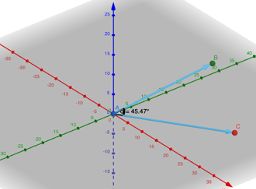
\includegraphics[width=7cm]{chapter_3/vector ex.png}
        \caption{แสดงตัวอย่างการหาเวกเตอร์ที่มีจุด A เป็นจุดร่วม}
    \end{figure}
    จากนั้นจึงหาองศาระหว่างเวกเตอร์ทั้งสองได้ จากสมการ
    \begin{equation}
        \alpha = \arccos{\left( \frac{\overrightarrow{AB} \cdot \overrightarrow{AC}}{|\overrightarrow{AB}| \cdot |\overrightarrow{AC}|} \right)}
    \end{equation}
    และเมื่อได้องศาเรียบร้อยแล้ว จึงจะนำไปตรวจสอบกับค่าที่ได้รับว่าตรงตามที่ได้กำหนดไว้หรือไม่ ซึ่งในส่วนนี้ได้กำหนดค่าความคลาดเคลื่อนเริ่มต้นที่ 10 องศา แต่สามารถเปลี่ยนแปลงได้ถ้ามีการระบุไว้ในไฟล์ข้อมูลท่าทาง
    \item คำสั่งตรวจสอบจุดใด ๆ ว่าอยู่ใกล้กันกับอีกจุดหนึ่งหรือไม่ จะรับจุดจำนวน 2 จุด แล้วทำการคำนวณว่าจุดที่ได้รับ อยู่ใกล้เคียงกันหรือไม่ โดยการสร้างทรงกลมขึ้นมาโดยให้จุดที่ได้รับเป็นจุดศูนย์กลาง จะได้ทรงกลมขึ้นมาทั้งหมด 2 ลูกที่รัศมีเท่า ๆ กัน แล้วจึงทำการคำนวณว่าทรงกลมนี้มีการทับกันบางส่วนหรือทั้งหมดหรือไม่ โดยถ้ามีการทับกันจะถือว่าจุดทั้งสองอยู่ใกล้เคียงกัน
\end{enumerate}

\subsection{ส่วนไฟล์ข้อมูลท่าทาง}
ไฟล์ข้อมูลท่าทาง จะเป็นไฟล์ที่รวบรวมข้อมูลท่าทางทั้งหมดของทั้งคอร์ส ซึ่งภายในจะประกอบไปด้วยข้อมูลลำดับของท่าทาง, วิธีการนับท่าทางเป็นการจับเวลาหรือการนับการกระทำซ้ำ, ที่อยู่ของสื่อที่จะนำมาใช้สอนผู้ใช้ และเกณฑ์ต่าง ๆ ที่จะต้องตรวจสอบท่าทางนั้น ๆ และจะใช้ภาษา YAML ในการใช้งาน ซึ่งจะแสดงโครงสร้างไฟล์เป็น UML Class Diagram ได้ดังนี้

\begin{figure}
    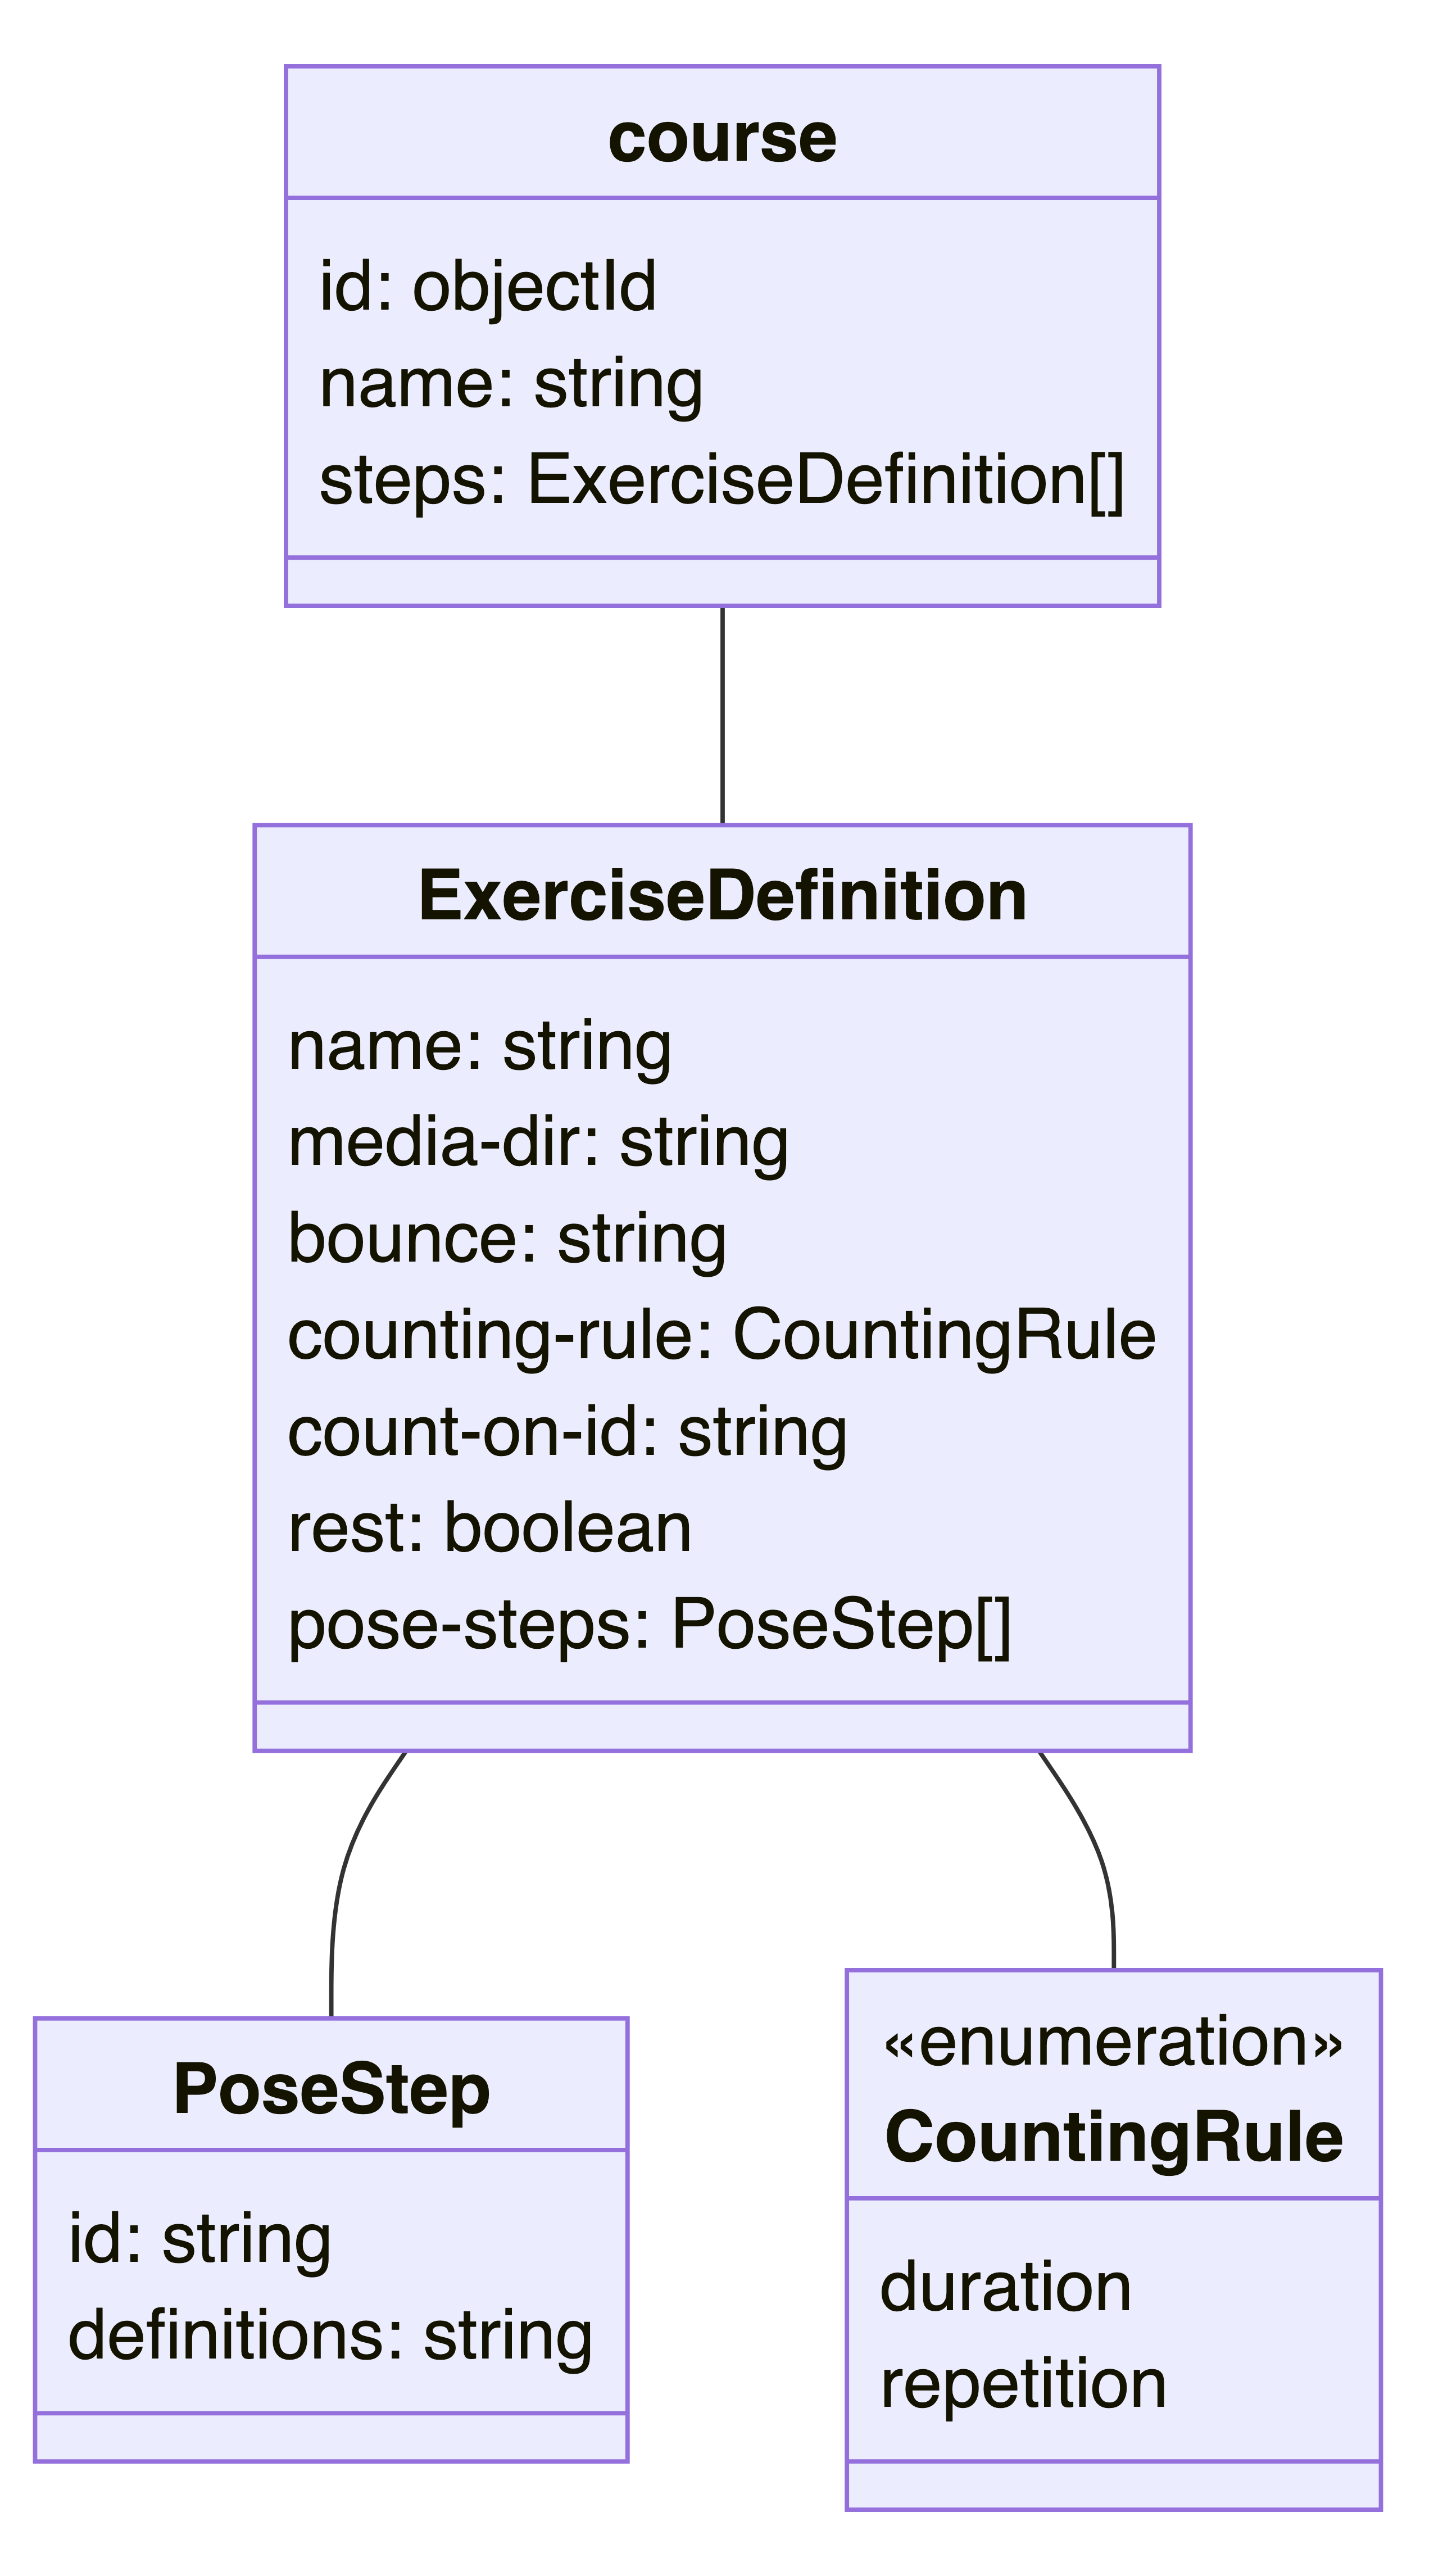
\includegraphics[width=6cm]{chapter_3/course-yaml-1.md.png}
    \caption{UML Class Diagram แสดงโครงสร้างไฟล์ข้อมูลท่าทาง}
\end{figure}

จากโครงสร้างไฟล์ จะมีรายละเอียดต่าง ๆ ในคลาส course ดังนี้
\begin{enumerate}
    \item id: ID ของคอร์ส
    \item name: ชื่อคอร์ส
    \item step: จะเป็นอาเรย์ใช้ในการเก็บข้อมูลท่าทางการออกกำลังกายทั้งหมด รวมถึงลำดับของท่าทางของการออกกำลังกายในคอร์ส ซึ่งจะใช้เก็บข้อมูลของคลาส ExerciseDefinition
\end{enumerate}

รายละเอียดของคลาส ExerciseDefinition มีดังนี้
\begin{enumerate}
    \item name: ชื่อท่าทาง
    \item media-dir: ที่อยู่ของสื่อที่จะนำมาใช้สอนผู้ใช้
    \item bounce: เป็นการกำหนดว่าท่าทางนี้เป็นแบบไป-กลับ หรือไม่ เช่น ในท่าทางวิดพื้นจะต้องมีการงอศอกลงและขึ้น ซึ่งจะต้องกำหนดให้เป็นท่าทางแบบไป-กลับ
    \item counting-rule: เป็นการกำหนดว่าจะใช้วิธีการนับแบบใด ซึ่งจะสามารถเลือกกำหนดได้ ระหว่างการจับเวลาหรือการนับการกระทำซ้ำ
    \item count-on-id: เป็นการกำหนด ID ของท่าทางย่อย ที่เมื่อผู้ใช้ทำท่าทางนี้สำเร็จจะให้นับจำนวนขึ้น ใช้ในกรณีที่ counting-rule ถูกกำหนดเป็นแบบการกระทำซ้ำเท่านั้น
    \item rest: ใช้กำหนดว่าในท่าทางนี้จะเป็นการพักหรือไม่ ถ้ากำหนดเป็น true ระบบจะไม่ทำการตรวจสอบท่าทางของผู้ใช้ เพื่อให้ผู้ใช้ได้พัก และจะไม่สนใจข้อมูลอื่น ๆ ที่ถูกกำหนด
    \item pose-steps: อาเรย์ที่ใช้อธิบายท่าทางย่อยในการออกกำลังกายนั้น ๆ
\end{enumerate}

รายละเอียดของคลาส PoseStep มีดังนี้
\begin{enumerate}
    \item id: ID ที่สามารถกำหนดได้อิสระ เพื่อใช้อ้างอิงถึงท่าทางนี้ใน count-on-id
    \item definitions: เกณฑ์ต่าง ๆ ที่จะต้องตรวจสอบในท่าทางย่อย ๆ นี้
\end{enumerate}
จากรายละเอียดข้างต้นในคลาส ExerciseDefinition จะมีการเก็บท่าทางย่อยใน key ชื่อ pose-steps ซึ่งในระบบจะมองว่าท่าทางการออกกำลังกายจะประกอบไปด้วยท่าทางย่อย ๆ ที่ต้องทำ เช่น ในการออกกำลังกายวิดพื้น จะมีท่าทางย่อย 2 ท่าทาง คือท่าทางเริ่มต้น และท่าทางเมื่องอศอก เป็นต้น โดยลำดับของท่าย่อย ๆ จะอ้างอิงตามลำดับในอาเรย์ ซึ่งถ้ามีการกำหนดให้ท่าทางนี้เป็นแบบไป-กลับ ระบบจะทราบว่าในท่าทางย่อย ๆ นี้เมื่อถึงท่าทางย่อยลำดับสุดท้ายแล้วผู้ใช้ต้องทำท่าทางย้อนกลับ

ในส่วนของคลาส PoseStep จะมี key ชื่อ definitions ซึ่งจะเป็น string ที่ใช้เก็บเกณฑ์ต่าง ๆ ที่จะต้องตรวจสอบในท่าทางย่อย ซึ่งจะมีคำสั่งดังนี้

\begin{enumerate}
    \item คำสั่ง “angle” เป็นคำสั่งตรวจสอบองศาของจุดที่ทำมุมกัน โดยจะมีการใช้งานดังนี้
    \begin{lstlisting}[caption=คำสั่ง angle]
        angle landmarkA landmarkB landmarkC {==|>|<|>=|<=|between|!between} angleA [angleB]
    \end{lstlisting}
    \indent ในคำสั่งนี้ ในขั้นแรกจะรับ Argument เข้ามา 3 ตัวซึ่งจะเป็นการระบุชื่อจุด Landmark ซึ่งจะแทนเป็นจุด A, B, C โดยชื่อ Landmark จะอ้างอิงจาก API ของ ML Kit จากนั้นจะเป็นการเลือกตัวดำเนินการว่าต้องการตรวจสอบองศาอย่างไร ซึ่งจะมีตัวเลือกเท่ากับ, มากกว่า, น้อยกว่า, มากกว่าหรือเท่ากับ, น้อยกว่าหรือเท่ากับ, อยู่ระหว่าง และไม่อยู่ระหว่าง และใน Argument สุดท้ายจะรับองศาที่ต้องการให้ตรวจสอบ ถ้าตัวดำเนินการได้ใช้เป็นแบบอยู่ระหว่างหรือไม่อยู่ระหว่าง จะต้องรับ Argument เพิ่มขึ้นมา ทำให้ต้องรับค่าองศา 2 ตัว เพื่อกำหนดขอบเขตองศาที่อยู่ระหว่างกัน
    \item คำสั่ง “touch” ซึ่งเป็นคำสั่งที่ใช้ในการตรวจสอบว่าจุด Landmark สองจุดอยู่ใกล้กันหรือไม่ โดยจะมีการใช้งาน ดังนี้
    \begin{lstlisting}[caption=คำสั่ง touch]
        touch landmarkA landmarkB
    \end{lstlisting}
    ในคำสั่งนี้จะรับ Argument เข้ามา 2 ตัว เป็นชื่อ Landmark ทั้งสองจุดที่ต้องการตรวจสอบ โดยชื่อ Landmark จะอ้างอิงจาก API ของ ML Kit
\end{enumerate}

\subsection{ส่วนการแนะนำท่าทางให้แก่ผู้ใช้}
เมื่อส่วนอัลกอริทึมการตรวจสอบท่าทางของผู้ใช้ ได้ประมวลผลท่าทางเรียบร้อยแล้ว ระบบจะส่งผลการตรวจสอบมายังส่วนการแนะนำท่าทางผู้ใช้ โดยจะทำการแปลงข้อมูลการตรวจสอบที่ได้ เป็นประโยคแนะนำท่าทางภาษาอังกฤษ เพื่อให้ผู้ใช้สามารถเข้าใจได้ง่าย และจะส่งผลลัพธ์การแนะนำท่าทางไปยังส่วนประสานงานผู้ใช้ เพื่อแสดงผลต่อไป